\documentclass[8pt]{beamer}
\usefonttheme[onlymath]{serif}


\setbeamertemplate{frametitle}{%
  \vskip1ex
  \usebeamerfont{frametitle}%
  \insertsubsectionhead\par        %  ← 원하는 대로 변경 가능
  \vskip1ex
  \hrule                             % 밑줄(선택)
}

% 테마 선택 (선택 사항)
% \usetheme{Madrid} % 기본 테마, 다른 테마 사용 가능
% \font{serif}
\usepackage{amsfonts}
\usepackage{amssymb}
\usepackage[T1]{fontenc} % To use combination of textbf, textit
\usepackage[dvipsnames]{xcolor}   % can use more variant colors

% \setcounter{MaxMatrixCols}{20}

% (필요한 패키지들)
% \usepackage{amsthm}
\setbeamertemplate{theorems}[numbered]  % 정리, 정의 등에 번호를 달아줌

% \theoremstyle{plain} % insert bellow all blocks you want in italic
% \newtheorem{theorem}{Theorem}[section] % to number according to section
% 
% \theoremstyle{definition} % insert bellow all blocks you want in normal text
% \newtheorem{definition}{Definition}[section] % to number according to section
% \newtheorem*{idea}{Proof idea} % no numbered block

\newtheorem{proposition}[theorem]{Proposition}

\usepackage{tcolorbox}

% 필요할 경우 패키지 추가
\usepackage{graphicx} % 이미지 삽입을 위한 패키지
\usepackage{amsmath}   % 수식 사용
\usepackage{hyperref}  % 하이퍼링크 추가
\usepackage{cleveref}
\usepackage{multicol}  % 여러 열 나누기
\usepackage{ulem} % 취소선 및줄 나누기
\usepackage{mathtools} % dcases
%\usepackage{xparse} % NewDocumentCommand



% \NewDocumentCommand{\DefThreeOp}{m}{%
%   % \csname #1\endcsname 라는 이름으로, 3개 인자를 받는 새 매크로를 정의
%   \expandafter\NewDocumentCommand\csname #1\endcsname{mmm}{%
%     \operatorname{#1}\!\bigl(##1,\,##2,\,##3\bigr)%
%   }%
% }

\newcommand{\mrm}[1]{\mathrm{#1}}
\newcommand{\mbb}[1]{\mathbb{#1}}
\newcommand{\mb}[1]{\mathbf{#1}}
\newcommand{\mc}[1]{\mathcal{#1}}
\newcommand{\tb}[1]{\textbf{#1}}
\newcommand{\ti}[1]{\textit{#1}}
\newcommand{\Pois}[1]{\operatorname{Pois}(#1)}

\newcommand{\myber}[1]{\operatorname{Bern}\!\left(#1\right)}
\newcommand{\Bin}[2]{\operatorname{Bin}\!\left(#1,#2\right)}
\newcommand{\NBin}[2]{\operatorname{NBin}\!\left(#1,#2\right)}
\newcommand{\mytoinf}[1]{#1 \rightarrow \infty}
\newcommand{\myexp}[1]{\exp{\left(#1\right)}}
\newcommand{\Unif}[2]{\operatorname{Unif}\!\left(#1, #2\right)}
\newcommand{\mygeom}[1]{\operatorname{Geom}\!\left(#1\right)}
\newcommand{\Expo}[1]{\operatorname{Expo}\!\left(#1\right)}
\newcommand{\abs}[1]{\left\lvert #1 \right\rvert}
\newcommand{\expec}[1]{\operatorname{E}\left[ #1 \right]}
\newcommand{\Var}[1]{\operatorname{Var}\left[#1\right]}
\newcommand{\myskew}[1]{\operatorname{Skew}\!\left[#1\right]}
\newcommand{\mykurt}[1]{\operatorname{Kurt}\!\left[#1\right]}
\newcommand{\mywei}[2]{\operatorname{Wei}\!\left(#1, #2\right)}
\newcommand{\Span}[1]{\operatorname{Span}\!\left(#1\right)}
\newcommand{\Cov}[2]{\operatorname{Cov}\!\left(#1, #2\right)}
\newcommand{\intinfty}{\int_{-\infty}^\infty}
\newcommand{\Corr}[2]{\operatorname{Corr}\!\left(#1, #2\right)}
\newcommand{\Mult}[3]{\operatorname{Mult}_{#1}\!\left(#2, #3\right)}
\newcommand{\Beta}[2]{\operatorname{Beta}\!\left(#1, #2\right)}
\newcommand{\HGeom}[3]{\operatorname{HGeom}\!\left(#1, #2, #3\right)}
\newcommand{\NHGeom}[3]{\operatorname{NHGeom}\!\left(#1,#2, #3\right)}
\newcommand{\GammaDist}[2]{\operatorname{Gamma}\!\left(#1, #2\right)}
%\DefThreeOp{PHGeom}


% 발표 제목, 저자, 날짜 설정
\title{Probability: Transformations}
\author{Gwanwoo Choi}
% \date{}

\begin{document}
% 표지 슬라이드

\begin{frame}
    \titlepage
\end{frame}

\subsection{Change of variables}
\begingroup
    \setbeamertemplate{frametitle}{%
    \vskip1ex
    \usebeamerfont{frametitle}%
    \insertframetitle\par        %  ← 원하는 대로 변경 가능
    \vskip1ex
    \hrule                             % 밑줄(선택)
    }
    \begin{frame}
        \frametitle{Table of Contents}
        \tableofcontents[currentsubsection]
    \end{frame}
\endgroup

% % 목차 슬라이드


\begin{frame}{.}
    \begin{itemize}
        \item There are so many situations in which we may be interested in non linear transformations
        \item Turning $X_1, \dots, X_n$ into the sum $T = X_1 + \cdots + X_n$ or sample mean $\bar{X}_n = T / n$ is a transformation from $\mbb{R}^n$ to $\mbb{R}$.
        \item The term for a sum of independent random variables is convolution, which are based on the law of total probability.
        \item Transformation that sorts observations turning $X_1, \dots, X_n$ into the order statistics $\min (X_1, \dots, X_n), \dots, \max (X_1, \dots, X_n)$ is a transformation from $\mbb{R}^n$ to $\mbb{R}^n$.
    \end{itemize}
\end{frame}

\begin{frame}{.}
    For some function $g$, how can we get the distribution of $g(X)$?

    \begin{itemize}
        \item Discrete case

            We can get PMF of $g(X) = Y$ by
            \[
                P(g(X) = Y) = \sum_{x:g(x) = y} P(X =x)
            \]

            Also, if $g$ is one-to-one function,

            \[
                P(g(X)=Y) = P(X = g^{-1}(y))
            \]
        \item Continuous Case

            If $g$ is strictly increasing,
            \[
                F_{g(X)}(y) = P(g(X) \leq y) = P(X \leq g^{-1}(y)) = F_X(g^{-1}(y))
            \]

            If $g$ is strictly decreasing,
            \[
                F_{g(X)} (y) = P(g(X) \leq y) = P(X > g^{-1}(y)) = 1 - F_X(g^{-1}(y))
            \]
    \end{itemize}
\end{frame}

\begin{frame}{.}

    \begin{theorem}{Change of variables in one dimension}
        Let $X$ be a continuous r.v. with PDF $f_x$, and $y = g(X)$, where $g$ is differentiable and strictly increasing (or strictly decreasing). Then the PDF of $Y$ is given by
        \[
        f_Y (y) = f_X (x) \abs{\frac{dx}{dy}}
        \]
        where $x = g^{-1}(y)$. The support of $Y$ is all $g(x)$ with $x$ in the support of $X$.
    \end{theorem}

    \begin{proof}
        Let $g$ be strictly increasing. The CDF of $Y$ is 
        \[
            F_Y(y) = P(Y \leq y) = P(g(X) \leq y) = P(X \leq g^{-1}(y)) = F_X(g^{-1}(y)) = F_X(x)
        \]
        So by the chain rule, the PDF of $Y$ is $f_Y(y) = f_X(x)\frac{dx}{dy}$.

        If $G$ be strictly decrasing, The CDF of $Y$ is 
        \[
            F_Y(y) = 1- F_X(g^{-1}(y))
        \]
        and PDF of $Y$ is $- f_X(x) \frac{dx}{dy} = f_X(x) \abs{\frac{dx}{dy}}$.
    \end{proof}
    It is easy to remember with $f_Y(y) dy = f_X(x)dx$ when $g$ is strictly increasing.
\end{frame}

\begin{frame}{.}
    \begin{example}{Log-Normal PDF}
        Let $X \sim \mc{N}(0,1)$, $Y = e^X$. Let's find the PDF of $Y$. Let $g(x) = e^x$, which is strictly increasing. The PDF of $X$ is $f_X(x) = \frac{1}{\sqrt{2\pi}} \exp{(x^2/2)}$. Then by the Change of variable theorem, $f_Y(y) = \frac{1}{\sqrt{2\pi}} \exp{(\log^2 y / 2)}\frac{1}{y}, \forall y \geq 0$.

        Also, we can obtain PDF of $Y$ via CDF.
        \[
        \begin{gathered}
            F_Y (y) = P(Y \leq y) = P(X \leq \log{y}) = \Phi(\log{y}) \\
            f_Y (y) = \varphi(\log (y)) \frac{1}{y}
        \end{gathered}
        \]
    \end{example}

    \begin{example}{Chi-Square PDF}
        Let $X \sim \mc{N}(0,1), Y = X^2$. The distribution of $Y$ is an example of a \tb{Chi-Square} distribution.

        \[
        \begin{gathered}
            F_Y(y) = P(X^2 \leq y) = P(-\sqrt{y} \leq X \sqrt{y}) = 2 \Phi(y) - 1 \\
            f_Y(y) = 2 \varphi(\sqrt{y}) \cdot \frac{1}{2} y^{-\frac{1}{2}}, \forall y>0
        \end{gathered}
        \]
    \end{example}
\end{frame}

\begin{frame}{.}
    \begin{example}[Lighthouse]
        Let $U \sim \Unif{-\frac{\pi}{2}}{\frac{\pi}{2}}$. Then the variable $X$ is defined by $X = \tanh{U}$. Find the distribution of $X$.

        By the Change of Variable, \[f_X(x) = f_U(u) \frac{du}{dx} = \frac{1}{\pi} \frac{1}{1+ x^2}\] which is same with Cauchy distribution.
    \end{example}

    \begin{theorem}[Change of Variables]
        Let $\mb{X} = (X_1, \dots ,X_n)$ be a continuous random vector with joint PDF $f_X$. Let $g: A_0 \to B_0$ and invertible function , where $A_0$ and $B_0$ are open subsets of $\mbb{R}^n$, $A_0$ contains the support of $\mb{X}$, and $B_0$ is the range of $g$.

        Let $\mb{Y} = g(\mb{X})$, and mirror this by letting $\mb{y} = g(\mb{X})$. Since $g$ is invertible, we also have $\mb{X} = g^{-1}(\mb{Y})$ and $\mb{x} = g^{-1}(\mb{y})$.

        Suppose that all the partial derivatives $\frac{\partial x_i}{\partial y_j}$ exists and are continuous. Assume that the determinant of this Jacobian matrix is never $0$. Then the joint PDF of $\mb{Y}$ is 
        \[
            f_{\mb{Y}}(\mb{y}) = f_{\mb{X}}(\mb{x}) (g^{\mb{-1}}(\mb{y})) \cdot \vert \abs{\frac{\partial \mb{x}}{\partial \mb{y}}} \vert
        \]
        And $0$ if determinant of jacobian is $0$.
    \end{theorem}
\end{frame}

\begin{frame}{.}
    \begin{example}[Box-Muller]
        Let $U \sim \Unif{0}{2\pi}$ and let $T \sim \Expo{1}$ be independent of $U$.
        Define
        \[
            X = \sqrt{2T} \cos{U}, Y = \sqrt{2T} \sin{U}
        \]
        Find the joint PDF of $(X,Y)$. Are they independent? What are their marginal distributions?

        Because $U$ and $T$ are independent, $f_{U,T}(u,t) = \frac{1}{2\pi}e^{-t}$.
        For $u \in (0, 2\pi)$ and $t >0$, 
        \[
            X^2 + Y^2 = 2T (\cos^2 U + \sin^2 U) = 2T
        \]

        Thus, $(X,Y)$ is expressed by cartesian coordinate from $(U,\sqrt{2T})$, polar coordinate.
        For vector $\mb{X} = (X,Y)$ and $\mb{Y} = (U,T)$, jacobian matrix $\frac{\partial \mb{x}}{\partial \mb{y}}$ is defined by 
        \[
        \frac{\partial \mb{x}}{\partial \mb{y}} = 
        \left(
            \begin{matrix}
                - \sqrt{2t} \sin u & \frac{1}{\sqrt{2t}} \cos u \\
                \sqrt{2t} \cos u & \frac{1}{\sqrt{2t}} \sin u
            \end{matrix}
        \right)
        \]
        And the determinant of Jacobian $\abs{\frac{\partial \mb{x}}{\partial \mb{y}}} = 1$
        \[
            f_{X,Y}(x,y) = f_{U,T} (u,t) = \frac{1}{2\pi} e^{-t} \vert \abs{\frac{\partial \mb{y}}{\partial \mb{x}}}\vert = \frac{1}{2\pi}e^{-t} = \frac{1}{\sqrt{2\pi}}e^{-x^2/2} \cdot \frac{1}{\sqrt{2\pi}} e^{-y^2/2}
        \]
        This result is called the \tb{Box-Muller} method for generating Normal r.v.s.
    \end{example}
\end{frame}

\subsection{Convolution}

\begingroup
    \setbeamertemplate{frametitle}{%
    \vskip1ex
    \usebeamerfont{frametitle}%
    \insertframetitle\par        %  ← 원하는 대로 변경 가능
    \vskip1ex
    \hrule                             % 밑줄(선택)
    }
    \begin{frame}
        \frametitle{Table of Contents}
        \tableofcontents[currentsubsection]
    \end{frame}
\endgroup

\begin{frame}{.}
    \begin{theorem}[Convolution sums and integrals]
        Let $X$ and $Y$ be independent r.v.s and $T=X+Y$ be their sum. If $X$ and $Y$ are discrete, then the PMF of $T$ is 
        \[
            P(T=t) = \sum_x P(Y=t-x) P(X=x) = \sum_y P(X=t-y)P(Y=y)
        \]

        If $X$ and $Y$ are continuous then the PDF of $T$ is
        \[
            f_T(t) = \int_{-\infty}^\infty f_Y(t-x) f_X(x) dx = \int_{-\infty}^\infty f_X(t-y) f_Y(y) dy
        \]
    \end{theorem}

    Proof for discrete
    \[
    \begin{aligned}
        P(T=t) &= \sum_x P(X+Y=t|X=x)P(X=x) \\
        &= \sum_x P(Y = t-x|X=x) P(X=x) \\
        &= \sum_x P(Y=t-x) P(X=x)
    \end{aligned}
    \]
\end{frame}


\begin{frame}{.}

    Proof for continuous

    \[
    \begin{aligned}
        F_T(t) &= P(X+Y \leq t) =\int_{-\infty}^\infty P(X+Y\leq t |X=x)f_X(x) dx \\
        &= \int_{-\infty}^\infty P(Y \leq t-x)f_X(x) dx = \int_{-\infty}^\infty F_Y(t-x)f_X(x)dx
    \end{aligned}
    \]
    
    PDF of $T$ can be obtained from above equation.
    \[
        f_T(t) = \int_{-\infty}^\infty f_Y(t-x)f_X(x)dx
    \]

    Proof with transformation.

    For random variable $X,Y$, let $T, W$ s.t. $T = X+Y, W=X$. Then $ \left[\begin{matrix}
    T \\ W
    \end{matrix}\right] = \left[\begin{matrix}
        1 & 1 \\ 1 & 0
    \end{matrix}\right] \left[\begin{matrix}
        X \\ Y
    \end{matrix}\right]$ holds and $|\abs{\frac{\partial (t,w)}{\partial (x,y)}}|=1$. Thus $f_{T,W}(t,w) = f_{X,Y}(x,y) = f_{X}(x) f_{Y}(y) = f_X(w) f_Y(t-w)$.

    \[
        f_T(t) = \int_{-\infty}^\infty f_{T,W}(t,w) dw = \int_{-\infty}^\infty f_X(x) f_Y(t-x) dx
    \]
\end{frame}

\begin{frame}{.}
    \begin{example}[Exponential convolution]
        Let $X,Y \overset{\text{i.i.d.}}{\sim} \Expo{\lambda}$. Find the distribution $T=X+Y$.
        \[
            \begin{aligned}
                f_T(t) &= \int_{-\infty}^\infty f_X(x) f_Y(t-x) dx = \int_{0}^t \lambda e^{-\lambda x} \cdot \lambda e^{-\lambda (t-x)} dx \\
                &= \lambda^2 \int_{0}^t e^{-\lambda t} dx = \lambda^2 t e^{-\lambda t}
            \end{aligned}
        \]
    \end{example}


    \begin{example}[Uniform Convolution]
        Let $X,Y \overset{\text{i.i.d.}}{\sim} \Unif{0}{1}$. Find the distribution of $T = X+Y$.

        \[
            f_T(t) = \int_{0}^t f_X(x) f_Y(t-x) dx =
            \begin{dcases}
                \int_{0}^t dx = t & \text{if } 0<t \leq 1 \\
                \int_{t-1}^1 dx = 2 - t & \text{if } 1<t<2 \\
            \end{dcases}
        \]
    \end{example}
\end{frame}

\subsection{Hypergeometric}

\begingroup
    \setbeamertemplate{frametitle}{%
    \vskip1ex
    \usebeamerfont{frametitle}%
    \insertframetitle\par        %  ← 원하는 대로 변경 가능
    \vskip1ex
    \hrule                             % 밑줄(선택)
    }
    \begin{frame}
        \frametitle{Table of Contents}
        \tableofcontents[currentsubsection]
    \end{frame}
\endgroup

\begin{frame}{.}
    \begin{example}[Vandermonde's identity]
        \[
            \binom{m+n}{k} = \sum_{j=0}^k \binom{m}{j} \binom{n}{k-j}
        \]
        Story proof : Consider a student organization consisting of $m$ juniors and $n$ seniors,  from which a committee of size $k$ will be chosen. 
        There are $\binom{m+n}{k}$ possibilities.
        If there are $j$ juniors in the committee, then there must be $ k-j$ seniors in the committee. 
        The right-hand side of the identity sums up the cases for $j$.
    \end{example}


\end{frame}


\begin{frame}{.}
    \begin{block}{Story: Hypergeometric distribution}
        Consider an urn with $w$ white balls and $b$ black balls. We draw $n$ balls out of the urn at random without replacement, such that all $\binom{w+b}{n}$ samples are equally likely. Let $X$ be the number of white balls in the sample. Then $X$ is said to have the \textbf{Hypergeometric distribution} with parameters $w,b,$ and $n$; we denote this by $X \sim \HGeom{w}{b}{n}$.

    \end{block}

    \begin{figure}
        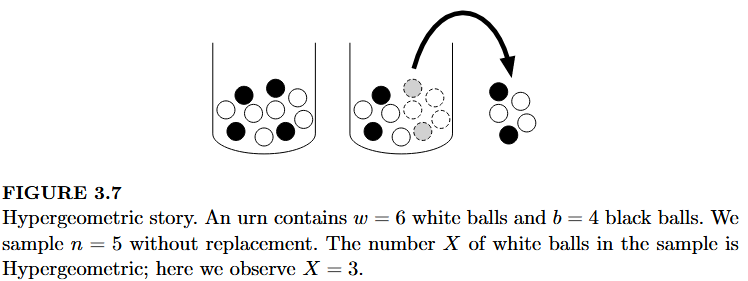
\includegraphics[width=0.8\textwidth]{HGeomFigure.png}
    \end{figure}
\end{frame}


\begin{frame}{.}
    \begin{theorem}[Hypergeometric PMF]
        If $X \sim \HGeom{w}{b}{n}$, then the PMF of $X$ is
        \[
            P(X=k) = \begin{dcases}
            \frac{\binom{w}{k} \binom{b}{n-k}}{\binom{w+b}{n}} & \text{if }  0\leq k \leq w, 0 \leq n-k \leq b \\
            0 & \text{otherwise}
            \end{dcases}
        \]
    \end{theorem}

    $\binom{w}{k}$ means $k$ white ball is chosen. $\binom{b}{n-k}$ means $n-k$ black ball is chosen.
    Denominator $\binom{w+b}{n}$ considers all the possibility for $k=0, \dots, n$.

    By the vandermonde's identity,  $\sum_{k=0}^n P(X=k)$ is $1$.

    So the PMF is valid.
\end{frame}

\begin{frame}{.}
    \begin{theorem}
        The $\HGeom{w}{b}{n}$ and $\HGeom{n}{w+b-n}{w}$ distributions are identical. That is, if $X \sim \HGeom{w}{b}{n}$, and $Y \sim \HGeom{n}{w+b-n}{w}$, then $X$ and $Y$ have the same distribution.
    \end{theorem}
    \begin{proof}
        We can proof this theorem with using the story. In $\HGeom{w}{b}{n}$, there exists two categories. White/Black and Sampled/Not-sampled. 
        \begin{itemize}
            \item  In first term $\HGeom{w}{b}{n}$, in total $w+b$ balls, first divide into white/black categories with $w$ number of white and $b$ number of black
            \item And second divide into sampled/not-sapmled categories with $n$ number of sampled and $w+b-n$ number of not-sampled.
            \item In the other hand, in $\HGeom{n}{w+b-n}{w}$, first divide into sampled/not-sampled categories, with $n$ number of sampled and $w+b-b$ number of not-sampled.
            \item And second divide into white/black cateogires with $w$ number of white and $b$ number of black.
        \end{itemize}
    \end{proof}
\end{frame}

\begin{frame}{.}
    Another proof is algebraic proof.

     \[
        \begin{gathered}
            P(X=k) = \frac{\binom{w}{k}\binom{b}{n-k}}{\binom{w+b}{n}} = \frac{w!b! n! (w+b-n)!}{k! (w-k)! (n-k)! (b-n+k)! (w+b)!} \\
            P(Y=k) = \frac{\binom{n}{k}\binom{w+b-n}{w-k}}{\binom{w+b}{w}} = \frac{w!b! n! (w+b-n)!}{k! (w-k)! (n-k)! (b-n+k)! (w+b)!}
        \end{gathered}
    \]

    \begin{definition}[Negative Hypergeometric distribution]
        An urn contains $w$ white balls and $b$ black balls, which are randomly drawn one by one \ti{without replacement}, until $r$ white balls have been obtained. 
        The number of black balls drawn before drawing the $r$th white ball has a \tb{Negative Hypergeometric} distribution with parameters $w, b, r$.

        We denote this distribution by $\NHGeom{w}{b}{r}$ ($r \leq w$).
        For example, if we shuffle a deck of cards and deal them one at a time, the number of cards dealt before uncovering the first ace is $\NHGeom{4}{48}{1}$.
    \end{definition}
\end{frame}

\begin{frame}{.}
    $X=K$ means that before the $r+k$th black ball is drawn, $k$ black balls and $r-1$ white balls are drawn.
    So, the PMF of $X \sim \NHGeom{w}{b}{r}$ is given by
    \[
        P(X=k)= \frac{\binom{w}{r-1} \binom{b}{k}}{\binom{w+b}{r+k-1}} \cdot \frac{w-r+1}{w+b-r-k+1}
    \]

    Another story for obtaining $P(X=k)$ is below. Imagine sort the $w$ white balls and $b$ black balls in oneline and draw balls one by one in the sorted order. Then among first $r+k-1$ balls there should exist $r-1$ white ball and $k$ black balls. Then among the last $w+b-r-k$ balls there should exist $w-r$ white balls.
    So the PMF is also given by
    \[
        P(X=k) = \frac{\binom{r+k-1}{r-1} \binom{w+b-r-k}{w-r}}{\binom{w+b}{w}}
    \]

\end{frame}

\subsection{Beta}

\begingroup
    \setbeamertemplate{frametitle}{%
    \vskip1ex
    \usebeamerfont{frametitle}%
    \insertframetitle\par        %  ← 원하는 대로 변경 가능
    \vskip1ex
    \hrule                             % 밑줄(선택)
    }
    \begin{frame}
        \frametitle{Table of Contents}
        \tableofcontents[currentsubsection]
    \end{frame}
\endgroup

\begin{frame}{.}
    \begin{itemize}
        \item The Beta distribution is a continuous distribution on the interval $(0, 1)$.
        \item It is a generalization of the $\Unif{0}{1}$ distribution, allowing the PDF to be non-constant on $(0,1)$.
    \end{itemize}

    \begin{definition}[Beta distribution]
        An r.v. $X$ is said to have the \tb{Beta distribution} with parameters $a$ and $b$, where $a > 0$ and $b > 0$, if its PDF is
        \[
            f(x) = \frac{1}{\beta (a,b)} x^{a-1} (1-x)^{b-1}, 0<x<1
        \]
        Where the constant $\beta(a,b)$ is chosen to make the PDF integrate to $1$. We write this as $X \sim \Beta{a}{b}$

        Note that $\beta(a,b)$ can be denoted by
        \[
            \beta(a,b) = \int_{0}^{1} x^{a-1} (1-x)^{b-1} dx
        \]
    \end{definition}

\end{frame}

\begin{frame}{.}
    \[
        f(x) = \frac{1}{\beta (a,b)} x^{a-1} (1-x)^{b-1}, 0<x<1
    \]
    \begin{columns}
        \begin{column}{0.4\textwidth}
            \begin{itemize}
                \item If $a=1$ and $b=1$, then $\Beta{1}{1} = \Unif{0}{1}$
                \item If $a<1$ and $b <1$, the PDF is U-shaped and opens upward.
                \item If $a>1$ and $a>1$, the PDF opens down.
                \item If $a=b$, the PDF is symmetric about $x= 0.5$.
                \item If $a>b$, the PDF favors values larger than $0.5$.
                \item If $a<b$, the PDF favors values smaller than $0.5$.
            \end{itemize}
        \end{column}

        \begin{column}{0.6\textwidth}
            \begin{figure}
                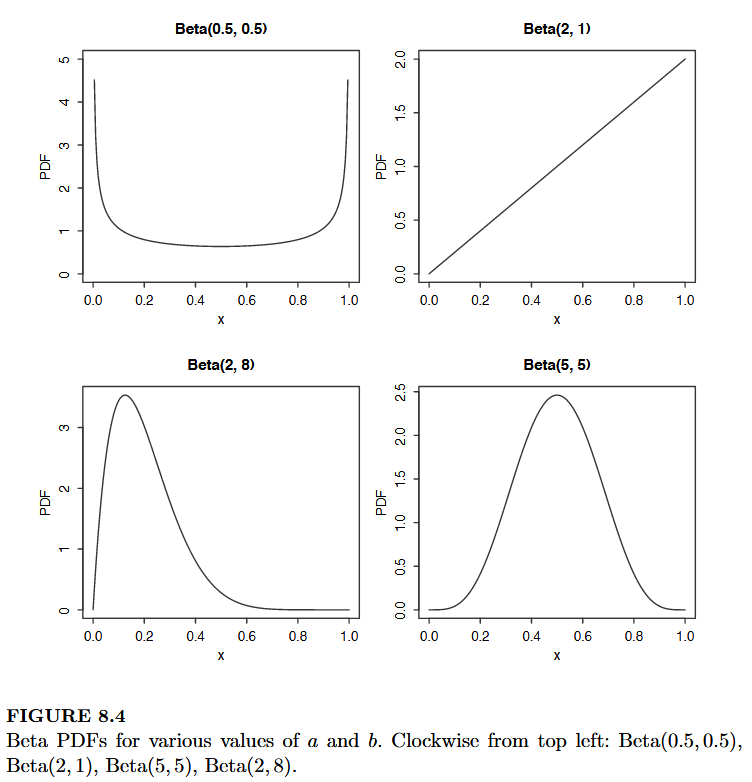
\includegraphics[width=1.0\textwidth]{BetaDists.png}
            \end{figure}
        \end{column}
    \end{columns}

\end{frame}

\begin{frame}{.}
    Generally, $\beta(a,b)$ needs some calculus to derive a general formula. But specially, if $a$ and $b$ are positive integers, we can easily calculate $\beta(a,b)$.

    \begin{block}{Story for $\beta(a,b)$ (Baye's billiards)}
        If $a,b$ are positive integers, then we can calculate $\beta(a,b)$ easier.

        Suppose there exists $n$ white balls and $1$ black balls.
        Then throw each ball into interval $(0,1)$ with probability $\Unif{0}{1}$ for position.

        Let denote the random variable $X$ for the number of white balls which is positioned left of black ball. Then the number of white ball which is positioned right of black ball is $n-k$.

        Let denote $P$, random variable for the position of black ball.

        The probability for $P(X=k)$ is defined by LOTP. $P(X=k) = \int_{0}^1 P(X=k|P=p) f_P(p) dp = \int_{0}^1 \binom{n}{k} p^k (1-p)^{n-k} dp$.

        Also, we can get the probability for $X=k$ with another story.

        Just throw whole $n+1$ white balls, and randomly make one of the ball color as black. Then the probability of $P(X=k) = \frac{1}{n+1}$.

        \begin{figure}
            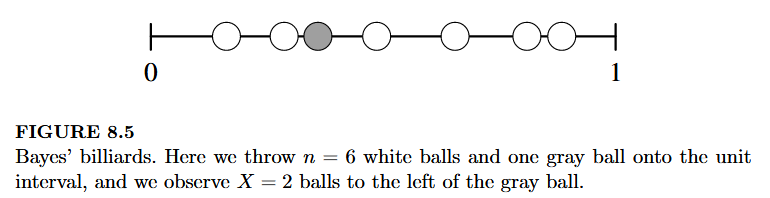
\includegraphics[width=0.9\textwidth]{BilliardsStoryBeta.png}
        \end{figure}
    \end{block}
\end{frame}

\begin{frame}{.}
    So from the two stories, we can notice that 
    \[
    \begin{gathered}
        \int_0^1 \binom{n}{k} x^{k} (1-x)^{n-k} dx = \frac{1}{n+1} \\
        \int^1_0 x^k (1-x)^{n-k} dx = \frac{k! (n-k)!}{(n+1) !}
    \end{gathered}
    \]

    By above equation, for positive integers $a,b$, with just replacing $k = a-1$ and $n-k = b-1$,
    \[
        \beta(a,b) = \int_0^1 x^{a-1} (1-x)^{b-1} = \frac{(a-1)! (b-1)!}{(a+b-1)!}
    \]

    So, when the $a,b$ are positive integers, then the PDF of $X$ is
    \[
        f_X(x) = \frac{(a-1)!(b-1)!}{(a+b-1)!} x^{a-1} (1-x)^{b-1}
    \]
\end{frame}

\begin{frame}{.}
    The Beta is a flexible family of distributions on $(0,1)$, and has many stories.

    \begin{block}{Story: Beta-Binomial conjugacy}
        We have a coin that lands Heads with probability $p$, but we don't know what $p$ is. Our goal is to infer the value of $p$ after observing the outcomes of $n$ tosses of the coin. The larger that $n$ is, the more accurately we should be able to estimate $p$.
    \end{block}

    Before starting the story, let introduce some pre-knowledges

    \begin{block}{pre-knowledge}
        \begin{itemize}
            \item Bayesian inference: in the Bayesian approach, treat the unknown probability $p$ as a random variable
            \item Prior distribution: distribution of $p$, $P(p)$
            \item Posterior distribution: With the result of experiment, as denoting random variable $X$ as the number of heads, $P(p|X)$
        \end{itemize}
    \end{block}

    Now, start the story. Let assume the prior distribution $P(p)$ is a Beta distribution. Let $p \sim \Beta{a}{b}$ for known constants $a$ and $b$. Then condition on knowing the value of $p$, $X|p \sim \Bin{n}{p}$. The marginal distribution of $X$ is called \tb{Beta-Binomial} distribution.

\end{frame}

\begin{frame}{.}
    By the Bayesian approach, since $X|p \sim \Bin{n}{p}$ and $p \sim \Beta{a}{b}$,
    \[
        f(p|X=k) = \frac{P(X=k|p)f(p)}{P(X=k)} = \frac{\binom{n}{k}p^{k} (1-p)^{n-k} \cdot \frac{1}{\beta(a,b)}p^{a-1} (1-p)^{b-1}}{P(X=k)}
    \]

    $P(X=k)$ can be obtained by marginalization.

    \[
        \begin{aligned}
        &P(X=k) = \int_{0}^1 P(X=k|p)f(p) dp= \int_0^1 \binom{n}{k} p^k (1-p)^{n-k} f(p) dp \\
        &= 
        \begin{dcases}
            \int_0^1 \binom{n}{k} p^k (1-p)^{n-k} dp = \frac{1}{n+1} & \text{if } a=1, b=1\\
           \NHGeom{}{}{} & \text{if } a,b \text{ are positive integers} 
        \end{dcases}
        \end{aligned}
    \]

    How can we calculate $f(p|X=k)$ when $a,b$ are real?
    Note that $f(p|X=k) \propto p^{a+k-1} (1-p)^{b+n-k-1}$.

    $\therefore p|X=k \sim \Beta{a+k}{b+n-k}$.

    Also, posterior $p|X=k$ becomes beta distribution.  From starting beta prior for r.v. $p$, and given binomial distribution for conditional r.v. $X=k|p$, Also we conclude that posterior distribution for r.v. $p|X=k$ is beta distribution. 

    This is called \tb{the Beta is the conjugate prior of the Binomial}.

\end{frame}

\subsection{Gamma}
\begingroup
    \setbeamertemplate{frametitle}{%
    \vskip1ex
    \usebeamerfont{frametitle}%
    \insertframetitle\par        %  ← 원하는 대로 변경 가능
    \vskip1ex
    \hrule                             % 밑줄(선택)
    }
    \begin{frame}
        \frametitle{Table of Contents}
        \tableofcontents[currentsubsection]
    \end{frame}
\endgroup

\begin{frame}{.}
    \begin{itemize}
        \item The Gamma distribution is a continuous distribution on the positive real line
        \item It is a generalization of the Exponential distribution
        \item While an Exponential r.v. represents the waiting time for the first success under conditions of memorylessness, we shall see that a Gamma r.v. represents the total waiting time for multiple successees.
    \end{itemize}

    Before writing down the PDF, let introduce \tb{gamma function}, a very famous function in mathematics that extends the factorial function beyond the realm of nonnegative integers.

    \begin{definition}[Gamma function]
        The \tb{Gamma function} $\Gamma$ is defined by
        \[
            \Gamma(a) = \int_0^\infty x^a e^{-x} \frac{dx}{x}, \forall a > 0
        \]
    \end{definition}

    Two important properties of gamma function
    \begin{itemize}
        \item $\Gamma(a+1) = a \Gamma(a), \forall a > 0$. $\Gamma(a+1) = \int_0^\infty x^a e^{-x} dx = \left[-x e^{-x}\right]^{-\infty}_0 + a \int_0^\infty x^{a-1} e^{-x} dx  \implies \Gamma(a+1) = a \Gamma(a)$
        \item $\Gamma(n) = (n-1)!$ if $n$ is a positive integer. Note that $\Gamma(1) = \int_0^\infty e^{-x} dx = 1$
    \end{itemize}
\end{frame}

\begin{frame}{.}
    From the gamma function, we can get
    \[
        1 = \int_{0}^{\infty} \frac{1}{\Gamma(a)} x^a e^{-x} \frac{dx}{x}
    \]
    Which is the valid PDF because integral for PDF satisfies $1$. We say that $X$ has $\GammaDist{a}{1}$ distribution if PDF $f_X(x) = \frac{1}{\Gamma(a)} x^{a}e^{-x}\frac{1}{x}, \forall x>0$.

    Let define $Y = X / \lambda$. Then by change of variable, 
    \[
        f_Y(y) = f_X(x) \abs{\frac{dx}{dy}} = \frac{1}{\Gamma(a)} (\lambda y)^a e^{-\lambda y} \frac{1}{\lambda y} \lambda = \frac{1}{\Gamma{a}} (\lambda y)^a e^{-\lambda y} \frac{1}{y}, \forall y >0
    \]

    \begin{definition}[Gamma distribution]
        An r.v. $Y$ is said to have the \tb{Gamma distribution} with parameters $a$ and $\lambda$ where $a >0$ and $\lambda >0$, if its PDF is
        \[
            f(y) = \frac{1}{\Gamma(a)} (\lambda y)^a e^{-\lambda y} \frac{1}{y}
        \]
    \end{definition}

    Taking $a=1$, then PDF of $Y \sim \GammaDist{1}{\lambda}$ becomes $f(y) = \lambda e^{-\lambda y}$, which is same PDF of $\Expo{\lambda}$. So $\GammaDist{1}{\lambda} = \Expo{\lambda}$.
\end{frame}

\begin{frame}{.}
    \begin{figure}
        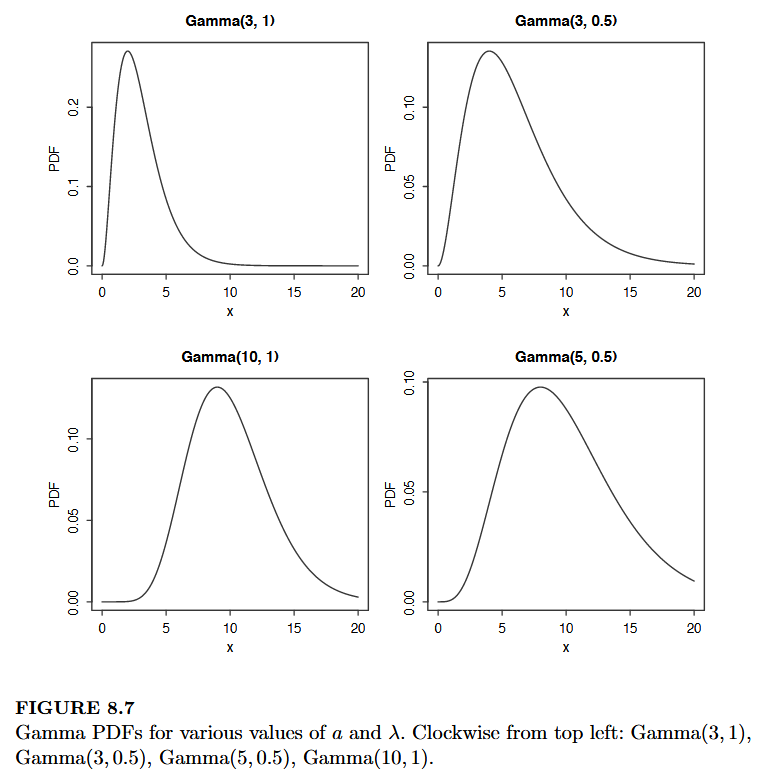
\includegraphics[width=0.7\textwidth]{GammaDistShapes.png}
    \end{figure}
\end{frame}

\begin{frame}{.}
    We can easily obtain moments of Gamma distribution.

    Let $X \sim \GammaDist{a}{1}$.

    \[
    \begin{gathered}
        \expec{X} = \int_0^\infty \frac{1}{\Gamma(a)} x^{a+1} e^{-x} \frac{dx}{x} = \frac{\Gamma(a+1)}{\Gamma(a)} = a \\
        \expec{X^2} = \int_0^\infty \frac{1}{\Gamma(a)} x^{a+2} e^{-x} \frac{dx}{x} = \frac{\Gamma(a+2)}{\Gamma(a)} = (a+1)a \\
        \Var{X} = \expec{X^2} - {\expec{X}}^2 = a^2 + a - a^2 = a \\
        \expec{X^c} = \int_0^\infty \frac{1}{\Gamma(a)} x^{a+c}e^{-x} \frac{dx}{x} = \frac{\Gamma(a+c)}{\Gamma(a)}, c>-a
    \end{gathered}
    \]

    Let $Y \sim \GammaDist{a}{\lambda}$

    \[
        \begin{gathered}
            \expec{Y} = \frac{1}{\lambda} \expec{X} = \frac{a}{\lambda} \\
            \Var{Y} = \frac{1}{\lambda^2} \Var{X} = \frac{a}{\lambda^2} \\
            \expec{Y^c} = \frac{1}{\lambda^c} \expec{X} = \frac{1}{\lambda^c}\frac{\Gamma(a+c)}{\Gamma(a)}, c>-a
        \end{gathered}
    \]
\end{frame}

\begin{frame}[allowframebreaks]{.}
    \begin{theorem}\label{thm:1}
        Let $X_1, \dots, X_n$ be i.i.d. $\Expo{\lambda}$. Then
        \[
            X_1 + \cdots + X_n \sim \GammaDist{n}{\lambda}
        \]
    \end{theorem}

    \begin{proof}
        The $\Expo{\lambda}$ MGF is $\frac{\lambda}{\lambda -t}, t<\lambda$, So the MGF of $X_1 + \cdots + X_n$ is $M_n(t) = (\frac{\lambda}{\lambda- t})^n$.

        Let $Y \sim \GammaDist{n}{\lambda}$.

        Then 
        \[
            \begin{aligned}
                \expec{e^{tY}}&=\int_0^\infty e^{ty} \frac{1}{\Gamma(n)} (\lambda y)^n e^{-\lambda y} \frac{dy}{y}\\
                &=\left(\frac{\lambda}{\lambda -t}\right)^n \int_0^\infty \frac{1}{\Gamma(n)} e^{-(\lambda -t)y} ((\lambda -t)y)^n \frac{dy}{y} \\
                &= \left(\frac{\lambda}{\lambda -t}\right)^n
            \end{aligned}
        \]

        So, MGF for $X_1 + \cdots + X_n$ and $Y$ are same.
    \end{proof}
\end{frame}

\begin{frame}{.}
    There exists another proof for theorem \ref{thm:1}.

    \begin{proof}
        Alternatively, we can compute the convolution integral inductively. 
        It suffices to consider the case $\lambda =1$.
        Let $T_n = X_1 + \cdots + X_n$.
        For $n=1$, $T_1 \sim \GammaDist{1}{1}$.
        Now suppose that $n=k, T_k \sim \GammaDist{k}{1}$ holds. Then
        $T_{k+1} = T_k +X_{n+1}$ and by convolutional integral

        \[
        \begin{aligned}
            \int_0^\infty f_{T_k}(x) f_{X_n}(t-x) dx&= \frac{1}{\Gamma(k)} \int_0^t x^{k-1} e^{-x} e^{-(t-x)} dx = \frac{e^t}{\Gamma(k)} \int_0^t x^{k-1} dx \\
            &= \frac{t^k e^{-t}}{\Gamma(k+1)}
        \end{aligned}
        \]
    \end{proof}

    So, below equations hold.
    \[
    \begin{gathered}
        \expec{Y} = \expec{X_1 + \cdots + X_a} = a \expec{X_1} = \frac{a}{\lambda} \\
        \Var{Y} = \Var{X_1 + \cdots + X_a} = a \Var{X_1} = \frac{a}{\lambda^2}
    \end{gathered}
    \]
\end{frame}

\begin{frame}{.}
    In the Chapter 5, Poission Process of each arrival time

    \begin{figure}
        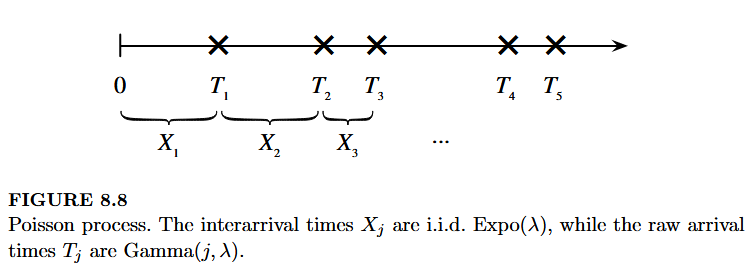
\includegraphics[width=0.8\textwidth]{ExpoAndGamma.png}
    \end{figure}

    \begin{itemize}
        \item Let $T_n$ be the $n$th arrival time. Then $T_1$ and each $T_{n+1} - T_n$ for $n\geq 1$ follows Poission distribution $\Pois{\lambda}$.
        \item Let $N_t$ is the number of emails that arrive at or before time $t$, then $T_n > t$ is the same event as $N_t < n $.
        \item So, by the upper theorem, $T_1 + (T_2 - T_1) + \dots + (T_n - T_{n-1}) = T_n \sim \GammaDist{n}{\lambda}$
        \item Gamma distribution represents an unknown \tb{rate} in a Poisson process because its support is $(0, \infty)$ (Otherwise, Beta distribution can represent an unknown probability of success because its support is $(0,1)$).
    \end{itemize}

\end{frame}

\begin{frame}{.}
    \begin{block}{Gamma-Poission conjugacy}
        In Blotchville, buses arrive at a certain bus stop according to a Poisson process with rate $\lambda$ buses per hour, where $\lambda$ is unknown. Based on his very memorable adventures in Blotchville, Fred quantifies his uncertainty about $\lambda$ using the prior $\lambda \sim \GammaDist{r_0}{b_0}$, where $r_0$ and $b_0$ are known, positive constants with $r_0$ an integer.

        To better understand the bus system, Fred wants to learn more about $\lambda$. He is a very patient person, and decides that he will sit at the bus stop for $t$ hours and count how many buses arrive in this time interval. Let $Y$ be the number of buses in this time interval, and suppose Fred observes $Y=y$.

        \begin{enumerate}
            \item Find Fred's hybrid joint distribution for $Y$ and $\lambda$.
            \item Find Fred's marginal distribution for $Y$.
            \item Find Fred's posterior distribution for $\lambda$, i.e., his conditional distribution of $\lambda$ given the data $y$.
            \item Find Fred's posterior mean $\expec{\lambda|Y=y}$ and posterior variance $\Var{\lambda|Y=y}$
        \end{enumerate}

        1. Find Fred's hybrid joint distribution for $Y$ and $\lambda$.

        Let $\lambda_0$ be the prior PDF of $\lambda$. The hybrid joint distributionof $Y$ and $\lambda$ is
        \[
            f(y, \lambda) = P(Y=y|\lambda) f_0(\lambda)= \frac{e^{-\lambda t}(\lambda t)^y}{y!} \frac{(b_0 \lambda)^{r_0} e^{-b_0 \lambda}}{\lambda \Gamma(r_0)}
        \]
    \end{block}
\end{frame}

\begin{frame}{.}
    2. Find Fred's marginal distribution for $Y$.

    To find the marginal distribution of $Y$,
    \[
    \begin{aligned}
        P(Y=y) &= \int_{-\infty}^\infty P(Y=y|\lambda) f_0(\lambda) d\lambda = \int_0^\infty \frac{e^{-\lambda t}(\lambda t)^y}{y!} \frac{(b_0 \lambda)^{r_0} e^{-b_0 \lambda}}{\lambda \Gamma(r_0)} d\lambda \\
        &= \frac{t^y b_0^{r_0}}{y! \Gamma(r_0)} \int_0^\infty \frac{\lambda^{(y + r_0)}e^{-\lambda(t + b_0)}}{\lambda} d\lambda \\
        &= \frac{\Gamma(r_0 + y)}{y! \Gamma(r_0)} \frac{t^y b_0^{r_0}}{(b_0 +t)^{(y+r_0)}} \int_0^\infty \frac{1}{\Gamma(r_0 + y)}((b_0 + t) \lambda)^{(y+r_0)} e^{-\lambda(b_0 + t)} \frac{d\lambda}{\lambda} \\
        &= \frac{(r_0 + y -1)!}{y! (r_0 -1)!} \left(\frac{b_0 }{b_0+t}\right)^{r_0} \left(\frac{t}{b_0 + t}\right)^{y}
    \end{aligned}
    \]
    Which is the negative binomial distribution, $\NBin{r_0}{\frac{b_0}{(b_0 + t)}}$, the number of failure before $r_0$ successes, in which the success probability is $\frac{b_0}{b_0+t}$
\end{frame}

\begin{frame}{.}
    3. Find Fred's posterior distribution for $\lambda$, i.e., his conditional distribution of $\lambda$ given the data $y$


    \[f(\lambda|Y=y) = \frac{P(Y=y|\lambda) f_0(\lambda)}{P(Y=y)} \]

    $P(Y=y)$ is just normalizing constant in terms of $\lambda$. so,
    \[
        f(\lambda | Y=y) \propto e^{-\lambda t} \lambda^{y} \lambda^{r_0} e^{-b_0 \lambda} \frac{1}{\lambda} = e^{-(b_0+t)\lambda} \lambda^{r_0+y} \frac{1}{\lambda}
    \]

    So, $\lambda \sim \GammaDist{r_0+y}{b_0 + t}$.

    When going from prior to posterior, the distribution of $\lambda$ stays in the Gamma family, so the Gamma is indeed the conjugate prior for the Poission.
\end{frame}

\subsection{Beta-Gamma connections}
\begingroup
    \setbeamertemplate{frametitle}{%
    \vskip1ex
    \usebeamerfont{frametitle}%
    \insertframetitle\par        %  ← 원하는 대로 변경 가능
    \vskip1ex
    \hrule                             % 밑줄(선택)
    }
    \begin{frame}
        \frametitle{Table of Contents}
        \tableofcontents[currentsubsection]
    \end{frame}
\endgroup

\begin{frame}{.}
    \begin{block}{Story. Bank-post office}
        While running errands, you need to go to the bank, then to the post office. Let $X \sim \GammaDist{a}{\lambda}$ be your waiting time in line at the bank, and let $Y \sim \GammaDist{b}{\lambda}$ be your waiting time in line at the post office (with the same $\lambda$ for both). Assume $X$ and $Y$ are independent. What is the joint distribution of $T=X+Y$ (your total wait at the bank and post office) and $W = \frac{X}{X+Y}$ (the fraction of your waiting time spent at the bank)?
    \end{block}

    Let $t=x+y$ and $w=\frac{x}{x+y}$. Then from $x = tw$ and $y=t(1-w)$, $\frac{\partial (x,y)}{\partial (t,w)} = \left[\begin{matrix}
        w & t \\ 1-w & -t
    \end{matrix}\right]$. By change of variable,

    
    \[
    \begin{aligned}
        f_{T,W}(t,w) &= f_{X,Y}(x,y) \vert \abs{\frac{\partial (x,y)}{\partial (t,w)}} \vert = f_X (x) f_Y(y) \vert \abs{\frac{\partial(x,y)}{\partial(t,w)}}\vert\\
        &= \frac{1}{\Gamma(a)} (\lambda x)^{a} e^{-\lambda x} \frac{1}{x} \frac{1}{\Gamma(b)} (\lambda y)^{b} e^{-\lambda y} \frac{1}{y} t \\
        &= \frac{1}{\Gamma(a)} (\lambda t w)^a e^{-\lambda t w} \frac{1}{tw} \frac{1}{\Gamma(b)} (\lambda t(1-w))^b e^{-\lambda t(1-w)} \frac{1}{t(1-w)} t \\
        &= \frac{\Gamma(a+b)}{\Gamma(a) \Gamma(b)} w^a  (1-w)^b \frac{1}{w} \frac{1}{(1-w)} \frac{1}{\Gamma(a+b)}(\lambda t)^{(a+b)} e^{-\lambda t} \frac{1}{t} \\
        &= \left(\frac{\Gamma(a+b)}{\Gamma(a) \Gamma(b)} w^{a-1} (1-w)^{b-1} \right) \left( \frac{1}{\Gamma(a+b)} (\lambda t)^{(a+b)} e^{-\lambda t} \frac{1}{t} \right)
    \end{aligned}
    \]
\end{frame}

\begin{frame}{.}
    For $0 < w< 1$ and $t>0$. The form of the joint PDF, together with Proposition 7.1.21, tells us several things
    \begin{itemize}
        \item Since the joint PDF factors into a function of $t$ times a function of $w$, we have that $T$ and $W$ are independent: the total waiting time is independent of the fraction of time spent at the bank.
        \item We recognize the marginal PDF of T and deduce that $T \sim \GammaDist{a+b}{\lambda}$
        \item The PDF of $W$ is $f_W(w) = \frac{\Gamma(a+b)}{\Gamma(a) \Gamma(b)} w^{a-1} (1-w)^{b-1}, 0<w<1$
    \end{itemize}

    So, $f_W(w)$ PDF is proportional to the $\Beta{a}{b}$ PDF, so it is the $\Beta{a}{b}$ PDF.
    Hence
    \[
        \frac{1}{\beta (a,b)} = \frac{\Gamma(a+b)}{\Gamma(a) \Gamma(b)}
    \]

    We can easily find the mean of $W \sim \Beta{a}{b}$ without the slightest trace of calculus.

    \[
        \begin{aligned}
            \expec{TW} &= \expec{T} \expec{W} \implies \expec{(X+Y) \cdot \frac{X}{X+Y}} = \expec{(X+Y)} \expec{\frac{X}{X+Y}} \\
            &\implies  \frac{\expec{X}}{\expec{X+Y}} = \expec{\frac{X}{X+Y}} = \expec{W} \implies \expec{W} = \frac{a/\lambda}{ a/\lambda + b/\lambda} = \frac{a}{a+b}
        \end{aligned}
    \]
\end{frame}

\begin{frame}{.}
    Or we can use some calculus to find moments of Beta distribution.
    \begin{example}[Exercise 8.30]
        Let $B \sim \Beta{a}{b}$. Use integration by pattern recognition to find $\expec{B^k}$ for positive integers $k$ and $\Var{B}$.
    \end{example}

    \[
    \begin{aligned}
        f_B(b) &= \int_0^1 \frac{\Gamma(a+b)}{\Gamma(a) \Gamma(b)} x^{a-1} (1-x)^{b-1} dx \implies \\
        \implies \expec{B^k} &= \int_0^1 \frac{\Gamma(a+b)}{\Gamma(a) \Gamma(b)} x^{a+k-1} (1-x)^{b-1} dx \\
        &= \frac{\Gamma(a+b)\Gamma(a+k)}{\Gamma(a+k+b) \Gamma(a)}\int_0^1 \frac{\Gamma(a+k+b)}{\Gamma(a+k) \Gamma(b)} x^{a+k-1} (1-x)^{b-1}dx \\
        &= \frac{(a+k-1)\cdots a}{(a+k+b-1)\cdots (a+b)}
    \end{aligned}
    \]
    So, $\expec{B} = \frac{a}{a+b}$ and $\expec{B^2} = \frac{(a+1)a}{(a+b+1)(a+b)}$. 
    \[
    \begin{aligned}
        \Var{B} &= \expec{B^2} - \expec{B}^2 = \frac{(a+1)a(a+b)}{(a+b+1)(a+b)(a+b)}  - \frac{a a (a+b+1)}{(a+b)(a+b)(a+b+1)} \\
        &= \frac{ab}{(a+b)^2 (a+b+1)}
    \end{aligned}
    \]
\end{frame}


\subsection{Order statistics}
\begingroup
    \setbeamertemplate{frametitle}{%
    \vskip1ex
    \usebeamerfont{frametitle}%
    \insertframetitle\par        %  ← 원하는 대로 변경 가능
    \vskip1ex
    \hrule                             % 밑줄(선택)
    }
    \begin{frame}
        \frametitle{Table of Contents}
        \tableofcontents[currentsubsection]
    \end{frame}
\endgroup

\begin{frame}{.}

    \begin{definition}[Order statistics]
        For r.v.s $X_1, X_2, \dots, X_n$, the \tb{order statistics} are the random variables $X_{(1)}, \dots, X_{(n)}$, where
        \[
            \begin{aligned}
                &X_{(1)} = \min (X_1, \dots, X_n) \\
                &X_{(2)} \text{ is the second-smallest among } X_1, \dots, X_n \\
                &\vdots \\
                &X_{(n-1)} \text{ is the second-largeest among } X_1, \dots, X_n \\
                &X_{(n)} = \max (X_1, \dots, X_n) \\
            \end{aligned}
        \]
        Note that $X_{(1)}\leq X_{(2)} \leq \dots \leq X_{(n)}$. We call $X_{(j)}$ the \tb{$j$th order statistic}. If $n$ is odd, $X_{(n+1)/2}$ is called the \tb{sample median} of $X_1, \dots, X_n$.
    
    \end{definition}

    \begin{itemize}
        \item The order statistics $X_{(1)}, \dots, X_{(n)}$ are r.v.s, and each $X_{(j)}$ is a function of $X_1, \dots, X_n$. 
        \item Even if the original r.v.s are independent, the order statistics are \tb{dependent}: If we know that $X_{(1)}=100$, then $X_{(n)}$ is forced to be at least $100$.
    \end{itemize}
\end{frame}

\begin{frame}{.}
    \begin{itemize}
        \item We will focus our attention on the case where $X_1, \dots, X_n$ are i.i.d. continuous r.v.s with CDF $F$ and PDF $f$.
        \item A complication we run into right away is that the transformation to order statistics is not invertible: Starting with $\min(X,Y)=3$ and $\max (X,Y)=5$, we can't tell whether the original values of $X$ and $Y$ were $3$ and $5$, respectively, or $5$ and $3$.
    \end{itemize}

    Let's start with the CDF of $X_{(n)} = \max(X_1, \dots, X_n)$.
    \[
    \begin{aligned}
        F_{X_{(n)}}(x) &= P(\max(x_1, \dots, X_n) \leq x) = P(X_1 \leq x, \dots, X_n \leq x) \\
        &= P(X_1 \leq x) \dots P(X_n \leq x) = (F(x))^n
    \end{aligned}
    \]
    
    Similarly, CDF of $X_{(1)}$ is obtained by 
    \[
        F_{X_{(1)}}(x) = 1- P(\min(X_1, \dots, X_n) > x) = 1- (1-F(x))^n
    \]
\end{frame}

\begin{frame}{.}
    \begin{figure}
        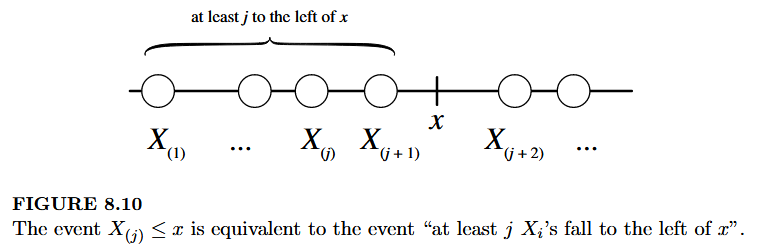
\includegraphics[width=0.85\textwidth]{OrderStatisticsCDF.png}
    \end{figure}
    The same logic lets us find the CDF of $X_{(j)}$. For the event $X_{(j)} \leq x$ to occur, we need at least $j$ of the $X_i$ to fall to the left of $x$.

    \[
    \begin{aligned}
        P(X_{(j)} \leq x) &= P(\text{at least }j \text{ of the }X_i\text{ are to the left of }x) 
        \\
        &=\sum_{k=j}^n \binom{n}{k} (F(x))^k (1-F(x))^{n-k}
    \end{aligned}
    \]
\end{frame}

\begin{frame}{.}
    \begin{figure}
        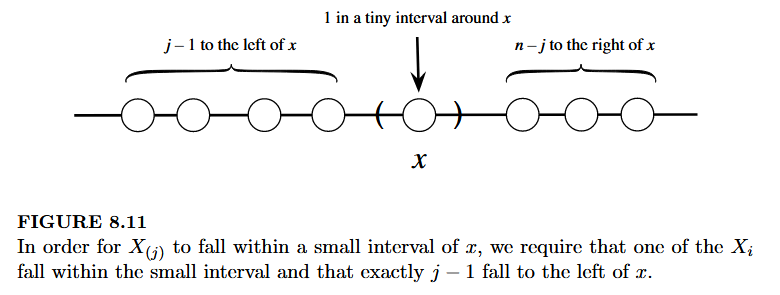
\includegraphics[width=0.85\textwidth]{OrderStatisticsPDF.png}
    \end{figure}

    \[
    \begin{aligned}
        &f_{X_{(j)}}(x) \Delta x = n f(x) \Delta x  \binom{n-1}{j-1} F(x)^{j-1} (1-F(x))^{n-j} \\
        &\implies f_{X_{(j)}} = n f(x) \binom{n-1}{j-1} F(x)^{j-1} (1-F(x))^{n-j}
    \end{aligned}
    \]
\end{frame}

\begin{frame}{.}
    \begin{example}[Order statistics in Uniforms]
        Let $U_1, \dots, U_n$ be i.i.d. $\Unif{0}{1}$. Then for $0 \leq x \leq 1, f(x) = 1$ and $F(x) = x$, so the PDF of $U_{(j)}$ is
        \[
            f_{U_{(j)}}(x) = n \binom{n-1}{j-1} x^{j-1} (1-x)^{n-j}
        \]
        $U_{(j)} \sim \Beta{j}{n-j+1}$ and $\expec{U_{(j)}} = \frac{j}{n+1}$.
        So, $\expec{\max(U_1, U_2)} = 2/3$ and $\expec{\min(U_1, U_2)} = 1/3$. This is the same result with example 7.2.2.
    \end{example}

\end{frame}

\end{document}